\documentclass[journal]{IEEEtran}
%\documentclass[12pt,journal,draftclsnofoot,onecolumn]{IEEEtran}
%\documentclass[conference]{IEEEtran}

\IEEEoverridecommandlockouts

\usepackage{etex}

%Fixing IEEEtran.cls bug with [english]{babel}
\makeatletter
\def\markboth#1#2{\def\leftmark{\@IEEEcompsoconly{\sffamily}\MakeUppercase{\protect#1}}%
\def\rightmark{\@IEEEcompsoconly{\sffamily}\MakeUppercase{\protect#2}}}
\makeatother

% \usepackage{t1enc}

\usepackage{listings}

%\usepackage[utf8x]{inputenc}
\usepackage[english]{babel}
\selectlanguage{english}
\usepackage{color}
\usepackage{lipsum}% http://ctan.org/pkg/lipsum
%\usepackage{caption}
\usepackage{cite}
\usepackage[pdftex]{graphicx}
%\usepackage{subfig}
%\usepackage{subcaption}
\usepackage{amsmath}
\usepackage{amsfonts}
\usepackage{array}
\usepackage{verbatim}
\usepackage{listings}
%\usepackage{algorithm}
%\usepackage{algorithmic}
%\usepackage{algpseudocode}
\usepackage{hyperref}
\usepackage{url}
\usepackage{enumerate}
\usepackage{multirow}

\usepackage{epsfig}
\usepackage{epstopdf}
\usepackage{multicol}% http://ctan.org/pkg/multicols
\usepackage[font=footnotesize]{caption}
\usepackage[font=scriptsize]{subcaption}
% Tikz
\usepackage{tikz}
\usepackage{pgfplots}
\pgfplotsset{compat=newest}
\pgfplotsset{plot coordinates/math parser=false}
\newlength\fheight
\newlength\fwidth
\usetikzlibrary{patterns,decorations.pathreplacing,backgrounds,calc}
\definecolor{SchoolColor}{RGB}{0.71, 0, 0.106}%181,0,27} unipd red
\definecolor{chaptergrey}{rgb}{0.61, 0, 0.09} % dialed back a little
\definecolor{midgrey}{rgb}{0.4, 0.4, 0.4}
\definecolor{chaptergreen}{rgb}{0.09, 0.612, 0}
\definecolor{chapterpurple}{rgb}{0.522, 0, 0.612}
\definecolor{chapterlightgreen}{rgb}{0, 0.612, 0.522}

%\raggedbottom

% Pseudocode
\usepackage{algorithm}
\usepackage[noend]{algpseudocode}
\renewcommand\algorithmicthen{}
\renewcommand\algorithmicdo{}
\usepackage{lscape}
\usepackage{setspace}

\addto\captionsenglish{\renewcommand{\figurename}{Fig.}}

\newcommand{\field}[1]{\mathbb{#1}}

\DeclareMathOperator*{\argmin}{arg\,min}
\DeclareMathOperator*{\argmax}{arg\,max}
\renewcommand{\arraystretch}{2}

\newcommand{\DP}[1]{\textbf{(DP: #1)}}
\newcommand{\el}[1]{\textr{(EL says: #1)}}
\newcommand{\fm}[1]{\texbf{(FM says: #1)}}

\usepackage{threeparttable}
%\usepackage[table,xcdraw]{xcolor}
\usepackage{tabularx}
   \usepackage{multirow}
   \usepackage{booktabs}
\newcommand{\tabitem}{~~\llap{\textbullet}~~}
   \usepackage{array, blindtext}
   \usepackage{wrapfig}
\usepackage{pdfpages}
\usepackage[acronym]{glossaries}

% use tikArchiviz images or eps
\newif\iftikz
\tikztrue

\graphicspath{{./figures/}}

\title{Heuristic optimization of Distributed Storage Network techniques}
\author{\IEEEauthorblockN{Federico Mason$^*$, Davide Peron$^*$, Enrico Lovisotto$^*$}\\
\small{{$^*$Department of Information Engineering, University of Padova -- Via Gradenigo, 6/b, 35131 Padova, Italy\\
Email: {\tt\{masonfed,perondav,lovisott\}@dei.unipd.it}\\}}
}

% Reduce the space below figs.
%\setlength{\belowcaptionskip}{-0.7cm}

%% Glossary
\newacronym{dsn}{DSN}{Distributed Storage Network}
\newacronym{edfc}{EDFC}{Exact Decentralized Fountain Codes}
\newacronym{adfc}{ADFC}{Approximate Decentralized Fountain Codes}
\newacronym{sa}{SA}{Simulated Annealing}
\newacronym{ga}{GA}{Genetic Algorithm}
\newacronym{jb}{JB}{Jumping Ball}
\newacronym{wsn}{WSN}{Wireless Sensor Network}
\newacronym{fp}{FP}{First Problem}
\newacronym{sp}{SP}{Second Problem}
\newacronym{of}{OF}{Objective Function}
\newacronym{cr}{CR}{Cooling Rate}
\newacronym{t}{T}{Temperature}
\newacronym{oc}{OC}{Old Candidate}
\newacronym{nc}{NC}{New Candidate}
\newacronym{sc}{SC}{Step Coefficient}
\newacronym{ac}{AC}{Acceptance Coefficient}
\newacronym{ap}{$P_A$}{Acceptance Probability}
\newacronym{ws}{$N_{WS}$}{Number of Worsening Steps}
\newacronym{wsmax}{$N_{WS}^{MAX}$}{ Maxiumum Number of Worsening Steps}

\glsresetall
\begin{document}

\setlength{\belowcaptionskip}{-0.2cm}

% reduce space after title
\makeatletter
\patchcmd{\@maketitle}
  {\addvspace{0.5\baselineskip}\egroup}
  {\addvspace{-1.2\baselineskip}\egroup}
  {}
  {}
\makeatother

\maketitle

\begin{abstract}
In some previous works about \gls{dsn}, two packet spreading algorithm are presented, \gls{edfc} and \gls{adfc}.

Unfortunately the tuning of their fundamental parameters, $x_d$ and $\nu(d)$ respectively, was not thoroughly investigated.

We try to perform such tuning applying some heuristic optimization techniques, such as \emph{Simulated Annealing} and \emph{Genetic Algorithm}, in order to explore the solution space of the problem.

\end{abstract}

\begin{IEEEkeywords}
Distributed Storage Networks, sensors, heuristic optimization
\end{IEEEkeywords}

\glsresetall
\label{sec:introduction}
We consider a \gls{wsn} whose nodes are distributed over a known region.
Some of them, called \textit{sensing nodes}, collect and deploy data from the environment (temperature, pressure, motion data, \ldots) while the others, called \textit{caching nodes}, simply store data coming from \textit{sensing nodes}.

In literature, a \gls{wsn} often has a central node, a powered sink connected to the internet.
Such special node receives all information collected by the nodes in the network and provides it to the users.

However, in our paper, following what has been done in \cite{Lin2007}, we get rid of this assumption.
Users then must collect the data stored in the network visiting the geographical region in which system is located.

In such a scenario, a randomly picked number of the nodes is visited by a user.
Our reference paper \cite{Lin2007}, guarantees source packets decodability using \emph{Random Fountain Codes}, combining and spreading $K$ source packets across $N$ total nodes such that, using any group of $K+\epsilon$ of them (with $\epsilon$ constant), the original information can be successfully retrieved with high probability.

The challenge here is to keep the communication cost at a minimum level, while keeping the failure probability low.

Traditional but expensive two-way packet delivery is then discarded, in favour of one-way \emph{random walks}, where only neighbours knowledge is required locally.
Random walks are designed according to \emph{Metropolis algorithm} such that the number of packets reaching each node resembles the Robust Soliton distribution, whose optimal decoding properties are known\cite{Luby}.

In this paper, we are going to find the optimal $x_d$ parameter for \gls{edfc} with three heuristic tecniques.
The optimal configurations are then tested with a network simulator, and further analysis is performed.

The article is structured in three sections.

In \autoref{sec:tech_approach} we present in detail the heuristic algorithms employed, first with a general description of the framework and then fucusing on our specific problem.

In \autoref{sec:results} we present the results obtained using the optimal parameter configuration in the simulator we have implemented.

\section{Technical Approach}
\label{sec:tech_approach}

The correct working of the algorithms \gls{edfc} and \gls{adfc} requires knowledge of $x_d$ and $\nu(d)$. $x_d$ is called \textit{redundancy coefficent} and is the solution of the following optimization problem.

\begin{equation}
	\label{firstproblem}
	\begin{split}
		minimize & \quad \sum_{d=1}^K x_d d \mu (d) \\
		subject \ to & \quad \begin{cases}
			Pr(Y<d|X=d) \leq \delta_d \\
			x_d \geq 1 \quad for \quad d = 1,...,K
		\end{cases}
	\end{split}
\end{equation}

$\nu(d)$ is a specific distribution and is the solution of the following optimization problem.

\begin{equation}
	\label{secondproblem}
	\begin{split}
		minimize & \quad \sum_{i=1}^{K/R}(\nu'(i)-\mu(i))^2 \\
		subject \ to & \quad \begin{cases}
			\sum_{i=1}^K \nu(i) = 1 \\
			\nu(i) \geq 0 \quad for \quad i=1,...,K
		\end{cases}
	\end{split}
\end{equation}

From now we call \ref{firstproblem} and \ref{secondproblem} simply \gls{fp} and \gls{sp}. The different parametrs that appear in \gls{fp} and in \gls{sp} are specified in ~\cite{Lin2007}. Both \gls{fp} and \gls{sp} have \textit{non-convex objective functions} and so it is impossible to determine the exact solution of these problems. To overcome this we build a series of heuristic algorithms.

The techniques we implement doesn't lead to exact solutions but to approximate solutions that are still optimal for our purposes. In particular these techniques are search algorithms that do not stop at the first localized local minimum. They continue to vary the outcome of the objective function, hoping to find a better local minimum than the one previously found.

\pagebreak

\subsection{Simulated Annealing}
The first algorithm that we have implemented is \gls{sa}. \gls{sa} is a probabilistic technique that takes ispiration from annealing in metallurgy, a process that aims to reduce materials defects.

In \gls{sa}, \gls{of} of the optimization problem is compared to the internal energy of a metallic material. Our algorithm is based on a parameter called \gls{t}. \gls{t} is initialized at a sufficient high value and then it is reduced until it reaches zero. Every new reduction of \gls{t} corresponds to a new step of the algorithm. At the first step the algorithm attribuites to the independent variable of \gls{of} a random value so that \gls{of} respects the constraints of the problem. This value becomes the \textit{candidate} to be the minimum value of \gls{of}. Then the \textit{candidate} is perturbed in an unique direction. If the new value found respect the constraints of \gls{of}, we keep it. If the new value found doesn't respect the constraints of \gls{of} we make a new perturbation. We call the process just described the search of a neighbour of the \textit{candidate}. Once a new admittable value of the \gls{of} is found, the algorithm has to establish if it want move to the neighbour of the \textit{candidate} or not. To make this decision \gls{sa} compares the value of \textit{oc} with the value of \textit{nc}.

 In case of \gls{nc} has better performance of \gls{oc}, that means that \gls{of} given by \gls{oc} is higher than \gls{of} given by \gls{nc}, the algorithm moves to \gls{nc} for sure. In case that \gls{nc} has worse performance than \gls{oc} the algorithm moves to \gls{nc} only with a certain probability that we call \textit{Acceptance Probability} $P_A$. This is done so that the algorithm has always the possibility to move away from a local minimum in search of a new solution. The value of the $P_A$ depends on the value of the dofference between the energy of \gls{nc} and the energy of \gls{oc} and is given in what follows.

 \begin{equation}
 	\label{accept_prob}
	P_A = \begin{cases}
		1 & \quad F(x_n)-F(x_o) < 0 \\
		e^{\psi(T)\cdot(F(x_n)-F(x_o))/T } & \quad F(x_n)-F(x_o) \geq 0
\end{cases}
 \end{equation}

In \ref{accept_prob} $x_n$ and $x_o$ represent the value of \gls{nc} and of \gls{oc} while $\psi(T)$ is a parameter depending on \gls{t} called \textit{Acceptance Coefficient}.

For every new value of \gls{t} the algorithm makes trys to move from the actual candidate a number of times equals to \textit{Steps Coefficient}. We note that \textit{Steps Coefficient} and the perturbation to which the candidates are subjected depend on \gls{t} as \textit{Acceptance Coefficient}. In particular all these paraeters decreases as the temperature decreases. This means that in initial steps of \gls{sa} is very easy for the result to change from the starting position while in the final steps is more likely that \gls{sa} stops at a local minimum.

When \gls{t} finally reach the zero values \gls{sa} esmines all the crossed candidates and returns the candidate with better performance.
It is therefore essential to always keep in mind the value of the best result going through right now.

\pagebreak

\begin{lstlisting}[frame=single]
T = Temperature
x = Candidate
Best_x = x
SC = Step coefficient
PA = Acceptance probability
while(T>0)
 for i = 1 to i = SC
  OC = x
  NC = Neighbour(x)
  while (NC doesn't respect costraints)
   NC = Neighbour(x)
  end
  with probability PA
   x = NC
  end
 end
T = get_new(Temperature)
SC = get_new(Step coefficent)
PA = get_new(PA)
if OF(x)<OF(Best_x)
 Best_x = x
end
end
return Best_x
\end{lstlisting} \captionof{lstlisting}{Simulated Alleaning} \label{code_sa}

\subsection{Jumping Ball}

The second technique that we implent is called \gls{jb}. \gls{jb} is a variant of \gls{sa} and it follows the same operating model. The only difference between \gls{jb} and \gls{sa} is that the searching for the best results could make a jump in some circumstannces. This jumps make the search of the candidate move along the function domain in a greater way than what happens in \gls{sa}.

Let's compare the code of \gls{sa} with the code of \gls{jb}. We note that have almost the same pattern. As in \gls{sa}, \gls{jb} uses the parameter \gls{t} which decrases as the algorithm goes on. At every new step \gls{t} is uptated as \gls{sc}, \gls{ac} and consequently \gls{ap}. For every new value of \gls{t} th algorithm moves throgh the domain of \gls{of} choosing new candidates.

Unlike \gls{sa}, \gls{jb} uses two more paramters that are called \gls{ws} and \gls{wsmax}. \gls{wsmax} is a fixed parameter while \gls{ws} changes value as the algorithm goes on. At the beginning the value of \gls{ws} is set to zero. Now we suppone that the algorithm moves to new caandidate with the probability \gls{ap}. If the new candidate has better performance than the previous one the values of \gls{ws} is immediately set to zero. Instead if the new candidate ha worse performance than the previous one the values of \gls{ws} in increase of one. Now we imagine that the algorithm moves for a great number of steps to candidate always worse than the previous one. In this case the value of \gls{ws} encreases al lot, untill it become close to \gls{wsmax}. When \gls{ws} beacomes greater than \gls{wsmax} the algorithm makes the jump. this mean that the searching of a new candidate doesn't happen as before. In particular the perturbation of the candidater is much bigger and does not envolve only one component of the candidate but a random number of them. Ina simply way we can say that the algorithm starts again the search froma point of the function domain very far from the previous one.

This happen in order to avoid that the lagoruthm moves to point of the function domain always worse than the point already crossed. 

\pagebreak

\begin{lstlisting}[mathescape=true,frame=single]
T = Temperature
x = Candidate
Best_x = x
SC = Step coefficient
PA = Acceptance probability
$ N_{WS} $ = 0
while(T>0)
 for i = 1 to i = SC
  OC = x
  NC = Neighbour(x)
  while (NC doesn't respect costraints)
   N_{WS} = N_{WS}+1
   if $N_{WS}<N_{WS}^{MAX}$
    NC = Neighbour(x)
   else
    NC = Jump(x)
    WS = 0
   end
  end
  with probability PA
   x = NC
  end
 end
T = get_new(Temperature)
SC = get_new(Step coefficent)
PA = get_new(PA)
$N_{WS}$ = 0
if OF(x)<OF(Best_x)
 Best_x = x
end
end
return Best_x
\end{lstlisting} \captionof{lstlisting}{Jumping ball}

\pagebreak

\begin{lstlisting}[frame=single]
\end{lstlisting} \captionof{lstlisting}{Genetic algorithm}


\subsection{Genetic Algorithm}
The third technique is called Genetic Algorithm.
The algorithm takes randomly an initial set of solution for the problem, called \textit{population}, and tries to evolve it toward better solutions.
Each candidate solution is called \textit{individual}, that is usually a multi-dimensional array. In biological applications, each component of the individual is a \textit{chromosome} or a \textit{genotype}, in our case it is simply an entry for the array.

\gls{ga} is an iterative process, in each iteration, the population is evolved in a new \textit{generation}.
In each generation, the objective function of each individual is evaluated. The best individuals (in terms of objective function) are selected and mutated to create the next generation.
The way in which an individual is mutated can be arbitrarily chosen.
Usually a single component is perturbated randomly, or parts of different solutions are joined togheter, to maintain the properties of the old solutions trying to improve it.

\section{Results}
\label{sec:results}
\begin{figure}
  \centering
	    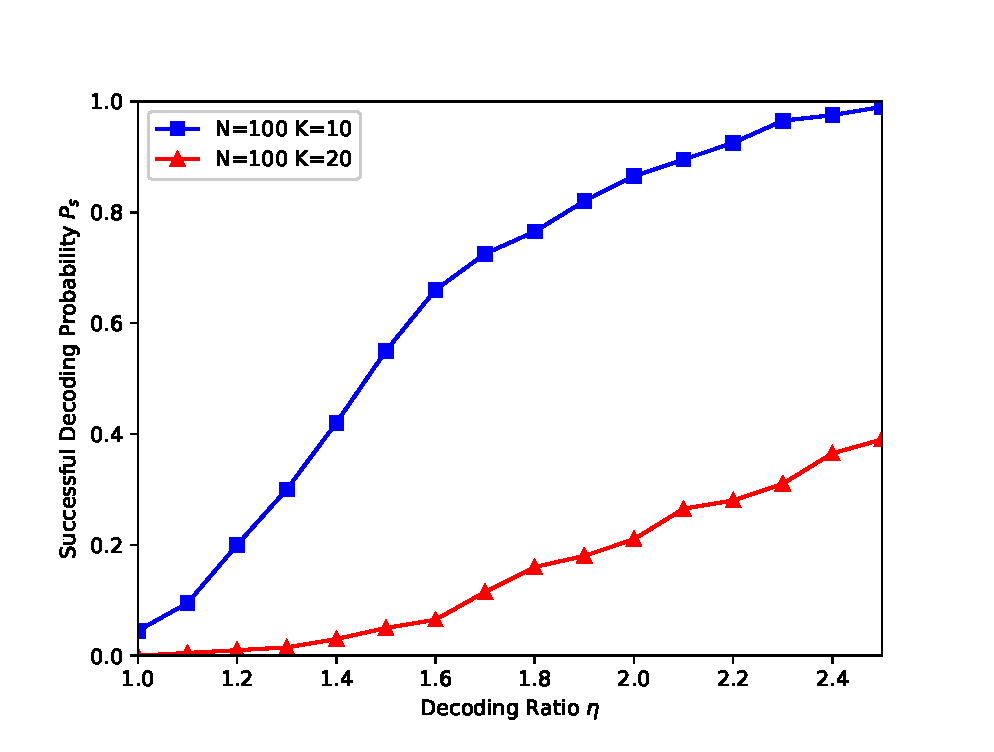
\includegraphics[width=0.9\columnwidth]{ratiovsprob.eps}
  \caption{Successfull decoding probability $P_s$ for different values of $N$, $K$ and decoding ratio $\nu$.}
  \label{fig:ratiovsprob}
\end{figure}

\section{Conclusions And Future Work}
\label{sec:conclusions}

\bibliographystyle{IEEEtran}
\bibliography{bibliography}

\end{document}
